\documentclass[../../dissertation.tex]{subfiles}
\begin{document}
The term \textit{random walk}, firstly introduced by \cite{kpearson1905}, is
classically defined as a stochastic process that models the path a walker would
take through a mathematical space, where each step made by the walker is
random. This can be used to model systems such as a molecule displaying
Brownian motion in a fluid, or even fluctuating stock prices as can be seen in
\cite{sottinen2001}.\par The simplest instance of this walk is on an infinite
discretely numbered line, whose mathmatical space is composed of integer
numbers. Here, the walker can only advance with equal probability in one of two
directions, depending on the outcome of a random event such as tossing a coin.
Starting from position $x=0$, the walker moves to $x = +1$ or $ x = -1$ with
$\frac{1}{2}$ probability after the first toss. On the second toss, the walker
could be on $x =\pm 2$ with $\frac{1}{4}$ probability each, and on $x = 0$ with
$\frac{1}{2}$.  Continuing this trend will result in a normal probability
distribution around the origin, as can be seen in the Python coding of figure
\ref{fig:MultClassicalWalk72180450}.
\begin{figure}[!h]
	%TODO: Decidir se faco outra fig para a evolucao do desvio padrao ou algo do genero. 
	\centering
	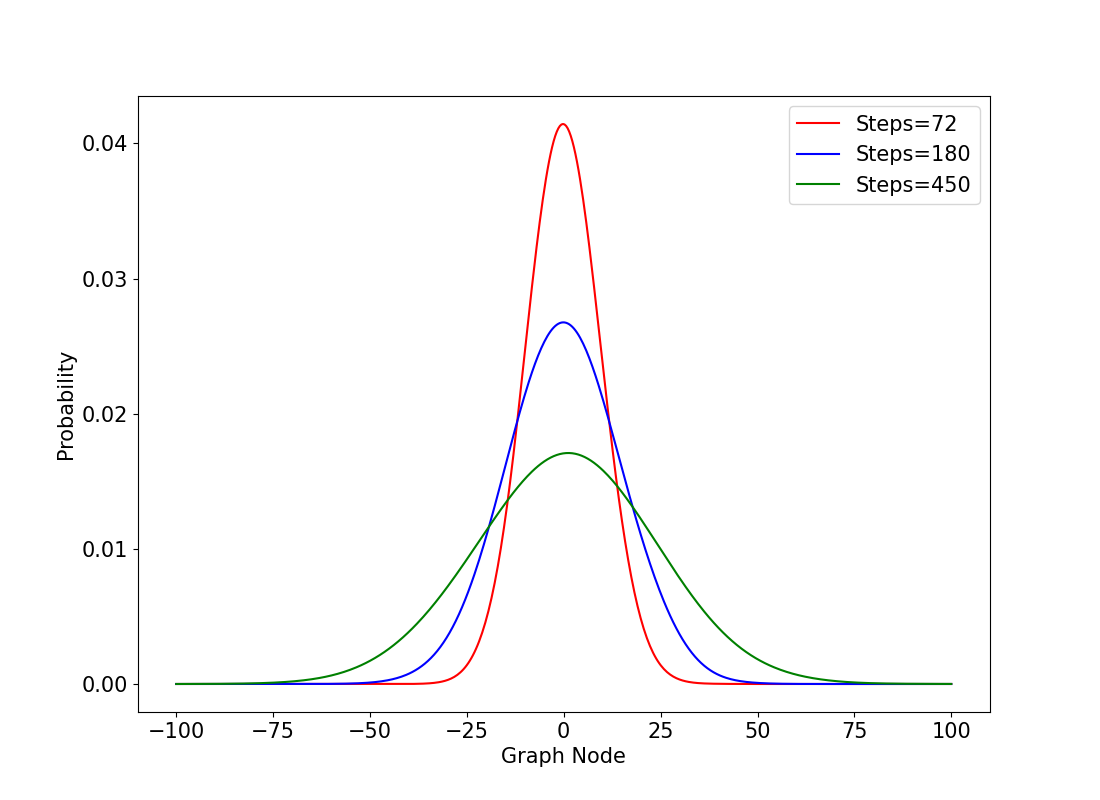
\includegraphics[scale=0.40]{img/ClassicalWalk/MultClassicalWalk72180450}
	\caption{Probability distribution for the classical random walk on a line, after $72$, $180$ and $450$, with starting position on vertex $0$.} 
	\label{fig:MultClassicalWalk72180450}
\end{figure}\par
%TODO: Decidir se menciono a equacao da probabilidade para explicar o facto de que a distribuicao e zero em t+n=impar, que e revelevante no coined quantum walk. Isto implica talvez ter que mencionar a probabilidade para as outras caminhadas, que nao sei se vale a pena. 
The number of iterations directly affects how far the walker can reach. As the number of
steps increases, the height of each curve at the starting position decreases
and the width of the curve increases. This relationship can be captured by the
\textit{position standard deviation}, and \cite{REN1} shows that the standard
deviation is
\begin{equation}
	\sigma(t) = \sqrt{t}.
	\label{eq:classicalWalkDeviation}
\end{equation}
%TODO: Talvez escrever mais um bocado nesta proxima linha.
In other words, equation \eqref{eq:classicalWalkDeviation} represents the rate at
which a walker moves away from the origin.\par
Note that this algorithm can be abstracted to graphs of higher dimensions. For
example, in a two dimensional lattice, a walker would be transversing a plane
with integer coordinates, choosing one of four directions in every
intersection. Notably, \cite{polya1921} proved that a walker in a two
dimensional lattice will almost surely return to the origin at some point.
However, the probability of returning to the origin decreases as the number of
dimensions increases, as shown by \cite{montrol1956} and \cite{finch2003}.
It is worth noting that a random walk, over a graph whose nodes are weighed and
directed, is analogous to a \textit{discrete-time Markov chain}\footnote{A
Markov chain can be described as a sequence of stochastic events where the the
probability of each event depends only on the state of the previous
event.}.
%TODO: \textcolor{red}{Você precisa esclarecer desde o início que está falando de uma caminhada clássica aqui, referenciar o livro do renato portugal, por exemplo, sobre o desvio padrão. Se quiser, pode fazer uma simulação clássica ou até mesmo abrir uma seção antes só para isso. Ah, precisa dizer que é uma linha infinita.}\par    
\end{document}
